\documentclass[a4paper, 10pt, final, garamond]{book}
\usepackage{cours-preambule}
\graphicspath{{./figures/}}

\makeatletter
\renewcommand{\@chapapp}{Contr\^ole de connaissances}
\makeatother

\setlist[blocQR,1]{leftmargin=10pt, resume, label=\sqenumi}

% \toggletrue{student}
% \HideSolutionstrue
% \toggletrue{corrige}
\renewcommand{\mycol}{black}

\begin{document}
\setcounter{chapter}{6}

\chapter{Chimie~: introduction\ifstudent{ (10')}}

\begin{enumerate}[label=\sqenumi, leftmargin=10pt]
	\nitem{1}%
	Indiquer, par un schéma, les trois états de la matière et le nom des
	transitions de phase possibles.
	\begin{center}
		\sswitch{
			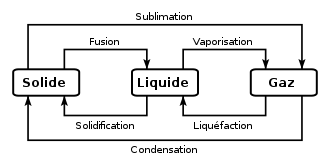
\includegraphics[width=.3\linewidth, draft=true]{trans_phase}
		}{
			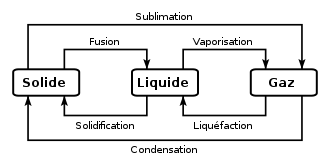
\includegraphics[width=.3\linewidth]{trans_phase}
		}
		\captionof{figure}{Vocabulaire transitions de phase}
	\end{center}
	\nitem{2}%
	Déterminer le nombre d'atomes de fer puis la quantité de matière de
	fer dans un clou de \SI{10}{g}. On donne $m_{\ce{Fe}} = \SI{9.37e-26}{kg}$ et
	$\Nc_A = \SI{6.022e23}{mol^{-1}}$.
	\smallbreak
	\vspace{-15pt}
	\wsw{
		\begin{gather*}
			\boxed{N = \frac{m}{m_{\rm Fe}}}
			\Lra
			\xul{N = \num{1.1e23}}
			\Lra
			\boxed{n = \frac{N}{\Nc_A}}
			\Lra
			\xul{n = \SI{1.8e-1}{mol}}
		\end{gather*}
	}
	\nitem{4}%
	L'air est constitué, en quantité de matière, à 80\% de diazote \ce{N2} et
	à 20\% de dioxygène \ce{O2}.
	\smallbreak
	On a
	$M(\ce{N_2}) = \SI{28.0}{g.mol^{-1}}$ et
	$M(\ce{O_2}) = \SI{32.0}{g.mol^{-1}}$.
	\smallbreak
	En déduire les fractions molaires puis les fractions massiques.
	\smallbreak
	\begin{isd}
		\wsw{
			On a
			\begin{gather*}
				n_{\tot} = n_{\ce{N_2}} + n_{\ce{O_2}}
				\qet
				m_{\tot} = m_{\ce{N_2}} + m_{\ce{O_2}}
			\end{gather*}
			Or, par lecture de l'énoncé on a
			\begin{gather*}
				x_{\ce{N_2}} = \frac{n_{\ce{N_2}}}{n_{\tot}} = \num{0.80}
				\qet
				x_{\ce{O_2}} = \frac{n_{\ce{O_2}}}{n_{\tot}} = \num{0.20}
			\end{gather*}
			Et par définition,
			\begin{align*}
				m_{\ce{N_2}} & = M(\ce{N_2})n_{\ce{N_2}} = M(\ce{N_2})x_{\ce{N_2}}n_{\tot}
				\\\text{et}\quad
				m_{\ce{O_2}} & = M(\ce{O_2})n_{\ce{O_2}} = M(\ce{O_2})x_{\ce{O_2}}n_{\tot}
			\end{align*}
		}
		\tcblower
		\wsw{
			\begin{align*}
				w_{\ce{N_2}}         & =
				\frac{
					M(\ce{N_2})x_{\ce{N_2}}\cancel{n_{\tot}}
				}{
					M(\ce{N_2})x_{\ce{N_2}}\cancel{n_{\tot}} +
					M(\ce{O_2})x_{\ce{O_2}}\cancel{n_{\tot}}
				}
				\\\Lra
				\Aboxed{w_{\ce{N_2}} & =
					\frac{
						M(\ce{N_2})x_{\ce{N_2}}
					}{
						M(\ce{N_2})x_{\ce{N_2}} +
						M(\ce{O_2})x_{\ce{O_2}}
					}
				}
				\\
				\makebox[0pt][l]{$\phantom{\AN}\xul{\phantom{w_{\ce{N_2}} = \num{0.78}}}$}
				\AN
				w_{\ce{N_2}}         & = \num{0.78}
				\\
				\text{et} \quad
				w_{\ce{O_2}}         & = 1-w_{\ce{N_2}}
				\\\Lra
				\Aboxed{w_{\ce{O_2}} & =
					\frac{
						M(\ce{O_2})x_{\ce{O_2}}
					}{
						M(\ce{N_2})x_{\ce{N_2}} +
						M(\ce{O_2})x_{\ce{O_2}}
					}
				}
				\\
				\makebox[0pt][l]{$\phantom{\AN}\xul{\phantom{w_{\ce{O_2}} = \num{0.22}}}$}
				\AN
				w_{\ce{O_2}}         & = \num{0.22}
			\end{align*}
		}
	\end{isd}
	\nitem{3}%
	On considère une seringue cylindrique de \SI{10}{cm} le long et de
	\SI{2.5}{cm} de diamètre, contenant \SI{0.250}{g} de diazote de masse
	molaire $M({\rm N}_2) = \SI{28.01}{g.mol^{-1}}$ à la
	température $T = \SI{20}{\degreeCelsius}$. On donne $R =
		\SI{8.314}{J.K^{-1}.mol^{-1}}$.
	\smallbreak
	\begin{isd}[sidebyside align=top]
		\begin{enumerate}
			\item Calculer le volume de la seringue
			\item Calculer la quantité de matière dans la seringue
			\item Calculer la pression exercée par le diazote dans la seringue
		\end{enumerate}
		\tcblower
		\wsw{
			\begin{enumerate}
				\item $\boxed{V = \pi \frac{d^{2}}{4}\times \ell} = \xul{\SI{49}{cm^{3}}}$
				\item $\boxed{n_{\ce{N_2}} = \frac{m_{\ce{N_2}}}{M(\ce{N_2})}} = \xul{\SI{8.93e-3}{mol}}$
				      \mitem
				      \begin{gather*}
					      \boxed{p=\frac{nRT}{V}}
					      \\
					      \qav
					      \left\{
					      \begin{array}{rcl}
						      n & = & \SI{8.93e-3}{mol}
						      \\
						      R & = & \SI{8.314}{J.mol^{-1}.K^{-1}}
						      \\
						      T & = & \SI{20}{\degreeCelsius} = \SI{293.15}{K}
						      \\
						      V & = & \SI{49}{cm^{3}} = \SI{49e-6}{m^{3}}
					      \end{array}
					      \right.\\
					      \AN
					      \xul{
						      p = \SI{4.4e5}{Pa} = \SI{4.4}{bars}
					      }
				      \end{gather*}
			\end{enumerate}
		}
		\vspace{-15pt}
	\end{isd}
	\vspace{-15pt}
\end{enumerate}

\ifstudent{
	\begin{tikzpicture}[remember picture, overlay]
		\node[anchor=north west, align=left]
		at ([shift={(1.4cm,0)}]current page.north west)
		{\\[5pt]\Large\bfseries Nom~:\\[10pt]\Large\bfseries Prénom~:};
		\node[anchor=north east, align=right]
		at ([shift={(-1.5cm,-17pt)}]current page.north east)
		{\Large\bfseries Note~:\hspace{1cm}/10};
	\end{tikzpicture}
}

\end{document}
